\documentclass[twoside]{book}

% Packages required by doxygen
\usepackage{fixltx2e}
\usepackage{calc}
\usepackage{doxygen}
\usepackage[export]{adjustbox} % also loads graphicx
\usepackage{graphicx}
\usepackage[utf8]{inputenc}
\usepackage{makeidx}
\usepackage{multicol}
\usepackage{multirow}
\PassOptionsToPackage{warn}{textcomp}
\usepackage{textcomp}
\usepackage[nointegrals]{wasysym}
\usepackage[table]{xcolor}

% NLS support packages
\usepackage[french]{babel}

% Font selection
\usepackage[T1]{fontenc}
\usepackage[scaled=.90]{helvet}
\usepackage{courier}
\usepackage{amssymb}
\usepackage{sectsty}
\renewcommand{\familydefault}{\sfdefault}
\allsectionsfont{%
  \fontseries{bc}\selectfont%
  \color{darkgray}%
}
\renewcommand{\DoxyLabelFont}{%
  \fontseries{bc}\selectfont%
  \color{darkgray}%
}
\newcommand{\+}{\discretionary{\mbox{\scriptsize$\hookleftarrow$}}{}{}}

% Page & text layout
\usepackage{geometry}
\geometry{%
  a4paper,%
  top=2.5cm,%
  bottom=2.5cm,%
  left=2.5cm,%
  right=2.5cm%
}
\tolerance=750
\hfuzz=15pt
\hbadness=750
\setlength{\emergencystretch}{15pt}
\setlength{\parindent}{0cm}
\setlength{\parskip}{0.2cm}
\makeatletter
\renewcommand{\paragraph}{%
  \@startsection{paragraph}{4}{0ex}{-1.0ex}{1.0ex}{%
    \normalfont\normalsize\bfseries\SS@parafont%
  }%
}
\renewcommand{\subparagraph}{%
  \@startsection{subparagraph}{5}{0ex}{-1.0ex}{1.0ex}{%
    \normalfont\normalsize\bfseries\SS@subparafont%
  }%
}
\makeatother

% Headers & footers
\usepackage{fancyhdr}
\pagestyle{fancyplain}
\fancyhead[LE]{\fancyplain{}{\bfseries\thepage}}
\fancyhead[CE]{\fancyplain{}{}}
\fancyhead[RE]{\fancyplain{}{\bfseries\leftmark}}
\fancyhead[LO]{\fancyplain{}{\bfseries\rightmark}}
\fancyhead[CO]{\fancyplain{}{}}
\fancyhead[RO]{\fancyplain{}{\bfseries\thepage}}
\fancyfoot[LE]{\fancyplain{}{}}
\fancyfoot[CE]{\fancyplain{}{}}
\fancyfoot[RE]{\fancyplain{}{\bfseries\scriptsize Généré le Samedi 26 Décembre 2015 12\+:26\+:15 pour Color Flood par Doxygen }}
\fancyfoot[LO]{\fancyplain{}{\bfseries\scriptsize Généré le Samedi 26 Décembre 2015 12\+:26\+:15 pour Color Flood par Doxygen }}
\fancyfoot[CO]{\fancyplain{}{}}
\fancyfoot[RO]{\fancyplain{}{}}
\renewcommand{\footrulewidth}{0.4pt}
\renewcommand{\chaptermark}[1]{%
  \markboth{#1}{}%
}
\renewcommand{\sectionmark}[1]{%
  \markright{\thesection\ #1}%
}

% Indices & bibliography
\usepackage{natbib}
\usepackage[titles]{tocloft}
\setcounter{tocdepth}{3}
\setcounter{secnumdepth}{5}
\makeindex

% Hyperlinks (required, but should be loaded last)
\usepackage{ifpdf}
\ifpdf
  \usepackage[pdftex,pagebackref=true]{hyperref}
\else
  \usepackage[ps2pdf,pagebackref=true]{hyperref}
\fi
\hypersetup{%
  colorlinks=true,%
  linkcolor=blue,%
  citecolor=blue,%
  unicode%
}

% Custom commands
\newcommand{\clearemptydoublepage}{%
  \newpage{\pagestyle{empty}\cleardoublepage}%
}


%===== C O N T E N T S =====

\begin{document}

% Titlepage & ToC
\hypersetup{pageanchor=false,
             bookmarks=true,
             bookmarksnumbered=true,
             pdfencoding=unicode
            }
\pagenumbering{roman}
\begin{titlepage}
\vspace*{7cm}
\begin{center}%
{\Large Color Flood }\\
\vspace*{1cm}
{\large Généré par Doxygen 1.8.10}\\
\vspace*{0.5cm}
{\small Samedi 26 Décembre 2015 12:26:15}\\
\end{center}
\end{titlepage}
\clearemptydoublepage
\tableofcontents
\clearemptydoublepage
\pagenumbering{arabic}
\hypersetup{pageanchor=true}

%--- Begin generated contents ---
\chapter{Index hiérarchique}
\section{Hiérarchie des classes}
Cette liste d\textquotesingle{}héritage est classée approximativement par ordre alphabétique \+:\begin{DoxyCompactList}
\item Callback\begin{DoxyCompactList}
\item \contentsline{section}{p8.\+demo.\+p8sokoban.\+Sokoban\+View}{\pageref{classp8_1_1demo_1_1p8sokoban_1_1_sokoban_view}}{}
\end{DoxyCompactList}
\item Runnable\begin{DoxyCompactList}
\item \contentsline{section}{p8.\+demo.\+p8sokoban.\+Sokoban\+View}{\pageref{classp8_1_1demo_1_1p8sokoban_1_1_sokoban_view}}{}
\end{DoxyCompactList}
\item Activity\begin{DoxyCompactList}
\item \contentsline{section}{p8.\+demo.\+p8sokoban.\+p8\+\_\+\+Sokoban}{\pageref{classp8_1_1demo_1_1p8sokoban_1_1p8___sokoban}}{}
\end{DoxyCompactList}
\item Surface\+View\begin{DoxyCompactList}
\item \contentsline{section}{p8.\+demo.\+p8sokoban.\+Sokoban\+View}{\pageref{classp8_1_1demo_1_1p8sokoban_1_1_sokoban_view}}{}
\end{DoxyCompactList}
\end{DoxyCompactList}

\chapter{Index des classes}
\section{Liste des classes}
Liste des classes, structures, unions et interfaces avec une brève description \+:\begin{DoxyCompactList}
\item\contentsline{section}{\hyperlink{classp8_1_1demo_1_1p8sokoban_1_1p8___sokoban}{p8.\+demo.\+p8sokoban.\+p8\+\_\+\+Sokoban} }{\pageref{classp8_1_1demo_1_1p8sokoban_1_1p8___sokoban}}{}
\item\contentsline{section}{\hyperlink{classp8_1_1demo_1_1p8sokoban_1_1_sokoban_view}{p8.\+demo.\+p8sokoban.\+Sokoban\+View} }{\pageref{classp8_1_1demo_1_1p8sokoban_1_1_sokoban_view}}{}
\end{DoxyCompactList}

\chapter{Documentation des classes}
\hypertarget{classp8_1_1demo_1_1p8sokoban_1_1p8___sokoban}{}\section{Référence de la classe p8.\+demo.\+p8sokoban.\+p8\+\_\+\+Sokoban}
\label{classp8_1_1demo_1_1p8sokoban_1_1p8___sokoban}\index{p8.\+demo.\+p8sokoban.\+p8\+\_\+\+Sokoban@{p8.\+demo.\+p8sokoban.\+p8\+\_\+\+Sokoban}}


Graphe d\textquotesingle{}héritage de p8.\+demo.\+p8sokoban.\+p8\+\_\+\+Sokoban\+:
\nopagebreak
\begin{figure}[H]
\begin{center}
\leavevmode
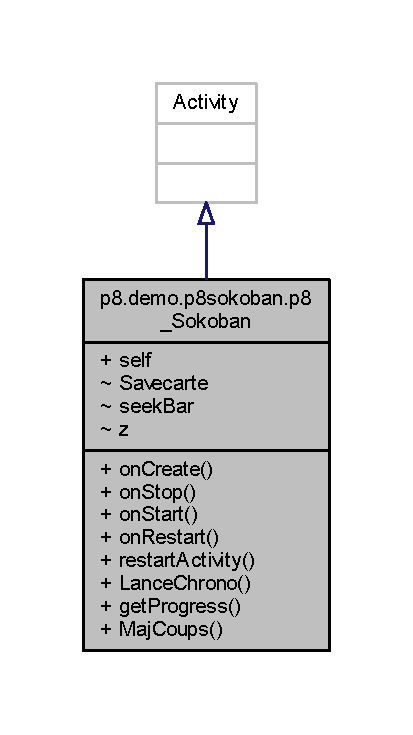
\includegraphics[width=198pt]{classp8_1_1demo_1_1p8sokoban_1_1p8___sokoban__inherit__graph}
\end{center}
\end{figure}


Graphe de collaboration de p8.\+demo.\+p8sokoban.\+p8\+\_\+\+Sokoban\+:
\nopagebreak
\begin{figure}[H]
\begin{center}
\leavevmode
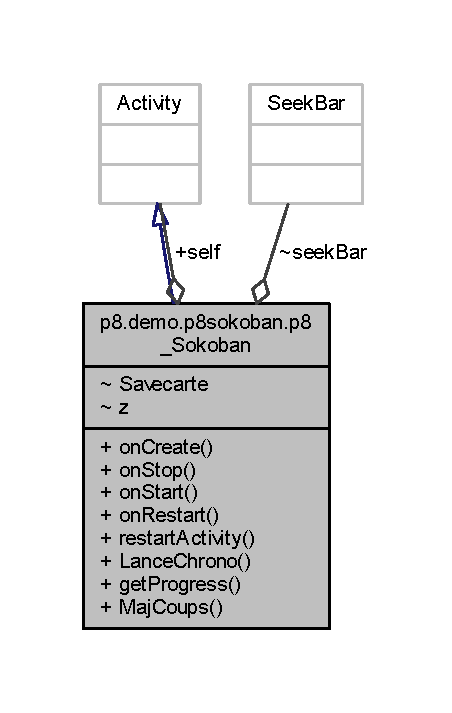
\includegraphics[width=217pt]{classp8_1_1demo_1_1p8sokoban_1_1p8___sokoban__coll__graph}
\end{center}
\end{figure}
\subsection*{Fonctions membres publiques}
\begin{DoxyCompactItemize}
\item 
void \hyperlink{classp8_1_1demo_1_1p8sokoban_1_1p8___sokoban_a4b9ef11394d277a9323ba41d191ebeaf}{on\+Create} (Bundle saved\+Instance\+State)
\item 
void \hyperlink{classp8_1_1demo_1_1p8sokoban_1_1p8___sokoban_a6b060c50b17932ba603624c5f2205344}{on\+Stop} ()
\item 
void \hyperlink{classp8_1_1demo_1_1p8sokoban_1_1p8___sokoban_af5bb8babf3e17336459cb12758eed269}{on\+Start} ()
\item 
void \hyperlink{classp8_1_1demo_1_1p8sokoban_1_1p8___sokoban_a8171d8ea7b1d39ab41354642f6d78534}{on\+Restart} ()
\end{DoxyCompactItemize}
\subsection*{Fonctions membres publiques statiques}
\begin{DoxyCompactItemize}
\item 
static void \hyperlink{classp8_1_1demo_1_1p8sokoban_1_1p8___sokoban_a956b703af9704745d8deffb1cf882249}{restart\+Activity} (Activity activity)
\item 
static void \hyperlink{classp8_1_1demo_1_1p8sokoban_1_1p8___sokoban_aba7394226cddb3359f918156472ac556}{Lance\+Chrono} ()
\item 
static int \hyperlink{classp8_1_1demo_1_1p8sokoban_1_1p8___sokoban_a75dbd4522cc44e46789299c7d52ba949}{get\+Progress} ()
\item 
static void \hyperlink{classp8_1_1demo_1_1p8sokoban_1_1p8___sokoban_a56fe9b42873640012e8b77d992a55480}{Maj\+Coups} ()
\end{DoxyCompactItemize}
\subsection*{Attributs publics statiques}
\begin{DoxyCompactItemize}
\item 
\hypertarget{classp8_1_1demo_1_1p8sokoban_1_1p8___sokoban_a872560ba71477fcbc9b7b878ecc9529e}{}static Activity {\bfseries self}\label{classp8_1_1demo_1_1p8sokoban_1_1p8___sokoban_a872560ba71477fcbc9b7b878ecc9529e}

\end{DoxyCompactItemize}


\subsection{Description détaillée}
Declaration de notre activity heritee de Activity 

\subsection{Documentation des fonctions membres}
\hypertarget{classp8_1_1demo_1_1p8sokoban_1_1p8___sokoban_a75dbd4522cc44e46789299c7d52ba949}{}\index{p8\+::demo\+::p8sokoban\+::p8\+\_\+\+Sokoban@{p8\+::demo\+::p8sokoban\+::p8\+\_\+\+Sokoban}!get\+Progress@{get\+Progress}}
\index{get\+Progress@{get\+Progress}!p8\+::demo\+::p8sokoban\+::p8\+\_\+\+Sokoban@{p8\+::demo\+::p8sokoban\+::p8\+\_\+\+Sokoban}}
\subsubsection[{get\+Progress()}]{\setlength{\rightskip}{0pt plus 5cm}static int p8.\+demo.\+p8sokoban.\+p8\+\_\+\+Sokoban.\+get\+Progress (
\begin{DoxyParamCaption}
{}
\end{DoxyParamCaption}
)\hspace{0.3cm}{\ttfamily [static]}}\label{classp8_1_1demo_1_1p8sokoban_1_1p8___sokoban_a75dbd4522cc44e46789299c7d52ba949}
Methode qui permet de recuperer la position de la seek\+Bar \begin{DoxyReturn}{Renvoie}

\end{DoxyReturn}
\hypertarget{classp8_1_1demo_1_1p8sokoban_1_1p8___sokoban_aba7394226cddb3359f918156472ac556}{}\index{p8\+::demo\+::p8sokoban\+::p8\+\_\+\+Sokoban@{p8\+::demo\+::p8sokoban\+::p8\+\_\+\+Sokoban}!Lance\+Chrono@{Lance\+Chrono}}
\index{Lance\+Chrono@{Lance\+Chrono}!p8\+::demo\+::p8sokoban\+::p8\+\_\+\+Sokoban@{p8\+::demo\+::p8sokoban\+::p8\+\_\+\+Sokoban}}
\subsubsection[{Lance\+Chrono()}]{\setlength{\rightskip}{0pt plus 5cm}static void p8.\+demo.\+p8sokoban.\+p8\+\_\+\+Sokoban.\+Lance\+Chrono (
\begin{DoxyParamCaption}
{}
\end{DoxyParamCaption}
)\hspace{0.3cm}{\ttfamily [static]}}\label{classp8_1_1demo_1_1p8sokoban_1_1p8___sokoban_aba7394226cddb3359f918156472ac556}
Methode qui permet de lancer le chronometre \hypertarget{classp8_1_1demo_1_1p8sokoban_1_1p8___sokoban_a56fe9b42873640012e8b77d992a55480}{}\index{p8\+::demo\+::p8sokoban\+::p8\+\_\+\+Sokoban@{p8\+::demo\+::p8sokoban\+::p8\+\_\+\+Sokoban}!Maj\+Coups@{Maj\+Coups}}
\index{Maj\+Coups@{Maj\+Coups}!p8\+::demo\+::p8sokoban\+::p8\+\_\+\+Sokoban@{p8\+::demo\+::p8sokoban\+::p8\+\_\+\+Sokoban}}
\subsubsection[{Maj\+Coups()}]{\setlength{\rightskip}{0pt plus 5cm}static void p8.\+demo.\+p8sokoban.\+p8\+\_\+\+Sokoban.\+Maj\+Coups (
\begin{DoxyParamCaption}
{}
\end{DoxyParamCaption}
)\hspace{0.3cm}{\ttfamily [static]}}\label{classp8_1_1demo_1_1p8sokoban_1_1p8___sokoban_a56fe9b42873640012e8b77d992a55480}
Methode qui permet de mettre a jour le nombre de coups effectue par le joueur en recuperant la position de la seek\+Bar, on met le nombre de coups maximum a une valeur fixe ensuite on affiche a l\textquotesingle{}ecran les valeurs en fonction de la progression du joueur \hypertarget{classp8_1_1demo_1_1p8sokoban_1_1p8___sokoban_a4b9ef11394d277a9323ba41d191ebeaf}{}\index{p8\+::demo\+::p8sokoban\+::p8\+\_\+\+Sokoban@{p8\+::demo\+::p8sokoban\+::p8\+\_\+\+Sokoban}!on\+Create@{on\+Create}}
\index{on\+Create@{on\+Create}!p8\+::demo\+::p8sokoban\+::p8\+\_\+\+Sokoban@{p8\+::demo\+::p8sokoban\+::p8\+\_\+\+Sokoban}}
\subsubsection[{on\+Create(\+Bundle saved\+Instance\+State)}]{\setlength{\rightskip}{0pt plus 5cm}void p8.\+demo.\+p8sokoban.\+p8\+\_\+\+Sokoban.\+on\+Create (
\begin{DoxyParamCaption}
\item[{Bundle}]{saved\+Instance\+State}
\end{DoxyParamCaption}
)}\label{classp8_1_1demo_1_1p8sokoban_1_1p8___sokoban_a4b9ef11394d277a9323ba41d191ebeaf}
Initialisation de l\textquotesingle{}activity avec le constructeur parent Charge le fichier main.\+xml comme vue de l\textquotesingle{}activite Recuperation de la vue cree a partir de son id Recuperation des widgets et autres avec les id Gestion de l\textquotesingle{}interface du jeu avec les evenements de la seekbar et des affichages dynamiques des textes 
\begin{DoxyParams}{Paramètres}
{\em saved\+Instance\+State} & \\
\hline
\end{DoxyParams}
\hypertarget{classp8_1_1demo_1_1p8sokoban_1_1p8___sokoban_a8171d8ea7b1d39ab41354642f6d78534}{}\index{p8\+::demo\+::p8sokoban\+::p8\+\_\+\+Sokoban@{p8\+::demo\+::p8sokoban\+::p8\+\_\+\+Sokoban}!on\+Restart@{on\+Restart}}
\index{on\+Restart@{on\+Restart}!p8\+::demo\+::p8sokoban\+::p8\+\_\+\+Sokoban@{p8\+::demo\+::p8sokoban\+::p8\+\_\+\+Sokoban}}
\subsubsection[{on\+Restart()}]{\setlength{\rightskip}{0pt plus 5cm}void p8.\+demo.\+p8sokoban.\+p8\+\_\+\+Sokoban.\+on\+Restart (
\begin{DoxyParamCaption}
{}
\end{DoxyParamCaption}
)}\label{classp8_1_1demo_1_1p8sokoban_1_1p8___sokoban_a8171d8ea7b1d39ab41354642f6d78534}
Quand on redemarre l\textquotesingle{}activity, on recupere la position de la seek\+Bar on stoppe et on redemarre le chronometre on relance aussi un nouveau thread pour pouvoir relancer une partie \hypertarget{classp8_1_1demo_1_1p8sokoban_1_1p8___sokoban_af5bb8babf3e17336459cb12758eed269}{}\index{p8\+::demo\+::p8sokoban\+::p8\+\_\+\+Sokoban@{p8\+::demo\+::p8sokoban\+::p8\+\_\+\+Sokoban}!on\+Start@{on\+Start}}
\index{on\+Start@{on\+Start}!p8\+::demo\+::p8sokoban\+::p8\+\_\+\+Sokoban@{p8\+::demo\+::p8sokoban\+::p8\+\_\+\+Sokoban}}
\subsubsection[{on\+Start()}]{\setlength{\rightskip}{0pt plus 5cm}void p8.\+demo.\+p8sokoban.\+p8\+\_\+\+Sokoban.\+on\+Start (
\begin{DoxyParamCaption}
{}
\end{DoxyParamCaption}
)}\label{classp8_1_1demo_1_1p8sokoban_1_1p8___sokoban_af5bb8babf3e17336459cb12758eed269}
Quand on demarre l\textquotesingle{}activity, on lance le jeu normalement avec un nouveau niveau \hypertarget{classp8_1_1demo_1_1p8sokoban_1_1p8___sokoban_a6b060c50b17932ba603624c5f2205344}{}\index{p8\+::demo\+::p8sokoban\+::p8\+\_\+\+Sokoban@{p8\+::demo\+::p8sokoban\+::p8\+\_\+\+Sokoban}!on\+Stop@{on\+Stop}}
\index{on\+Stop@{on\+Stop}!p8\+::demo\+::p8sokoban\+::p8\+\_\+\+Sokoban@{p8\+::demo\+::p8sokoban\+::p8\+\_\+\+Sokoban}}
\subsubsection[{on\+Stop()}]{\setlength{\rightskip}{0pt plus 5cm}void p8.\+demo.\+p8sokoban.\+p8\+\_\+\+Sokoban.\+on\+Stop (
\begin{DoxyParamCaption}
{}
\end{DoxyParamCaption}
)}\label{classp8_1_1demo_1_1p8sokoban_1_1p8___sokoban_a6b060c50b17932ba603624c5f2205344}
Quand on stoppe l\textquotesingle{}activity, on sauvegarde la grille lorsqu\textquotesingle{}on arretes l\textquotesingle{}application \hypertarget{classp8_1_1demo_1_1p8sokoban_1_1p8___sokoban_a956b703af9704745d8deffb1cf882249}{}\index{p8\+::demo\+::p8sokoban\+::p8\+\_\+\+Sokoban@{p8\+::demo\+::p8sokoban\+::p8\+\_\+\+Sokoban}!restart\+Activity@{restart\+Activity}}
\index{restart\+Activity@{restart\+Activity}!p8\+::demo\+::p8sokoban\+::p8\+\_\+\+Sokoban@{p8\+::demo\+::p8sokoban\+::p8\+\_\+\+Sokoban}}
\subsubsection[{restart\+Activity(\+Activity activity)}]{\setlength{\rightskip}{0pt plus 5cm}static void p8.\+demo.\+p8sokoban.\+p8\+\_\+\+Sokoban.\+restart\+Activity (
\begin{DoxyParamCaption}
\item[{Activity}]{activity}
\end{DoxyParamCaption}
)\hspace{0.3cm}{\ttfamily [static]}}\label{classp8_1_1demo_1_1p8sokoban_1_1p8___sokoban_a956b703af9704745d8deffb1cf882249}
Methode qui permet de redemarrer l\textquotesingle{}activity 
\begin{DoxyParams}{Paramètres}
{\em activity} & \\
\hline
\end{DoxyParams}


La documentation de cette classe a été générée à partir du fichier suivant \+:\begin{DoxyCompactItemize}
\item 
app/src/main/java/p8/demo/p8sokoban/p8\+\_\+\+Sokoban.\+java\end{DoxyCompactItemize}

\hypertarget{classp8_1_1demo_1_1p8sokoban_1_1_sokoban_view}{}\section{Référence de la classe p8.\+demo.\+p8sokoban.\+Sokoban\+View}
\label{classp8_1_1demo_1_1p8sokoban_1_1_sokoban_view}\index{p8.\+demo.\+p8sokoban.\+Sokoban\+View@{p8.\+demo.\+p8sokoban.\+Sokoban\+View}}


Graphe d\textquotesingle{}héritage de p8.\+demo.\+p8sokoban.\+Sokoban\+View\+:
\nopagebreak
\begin{figure}[H]
\begin{center}
\leavevmode
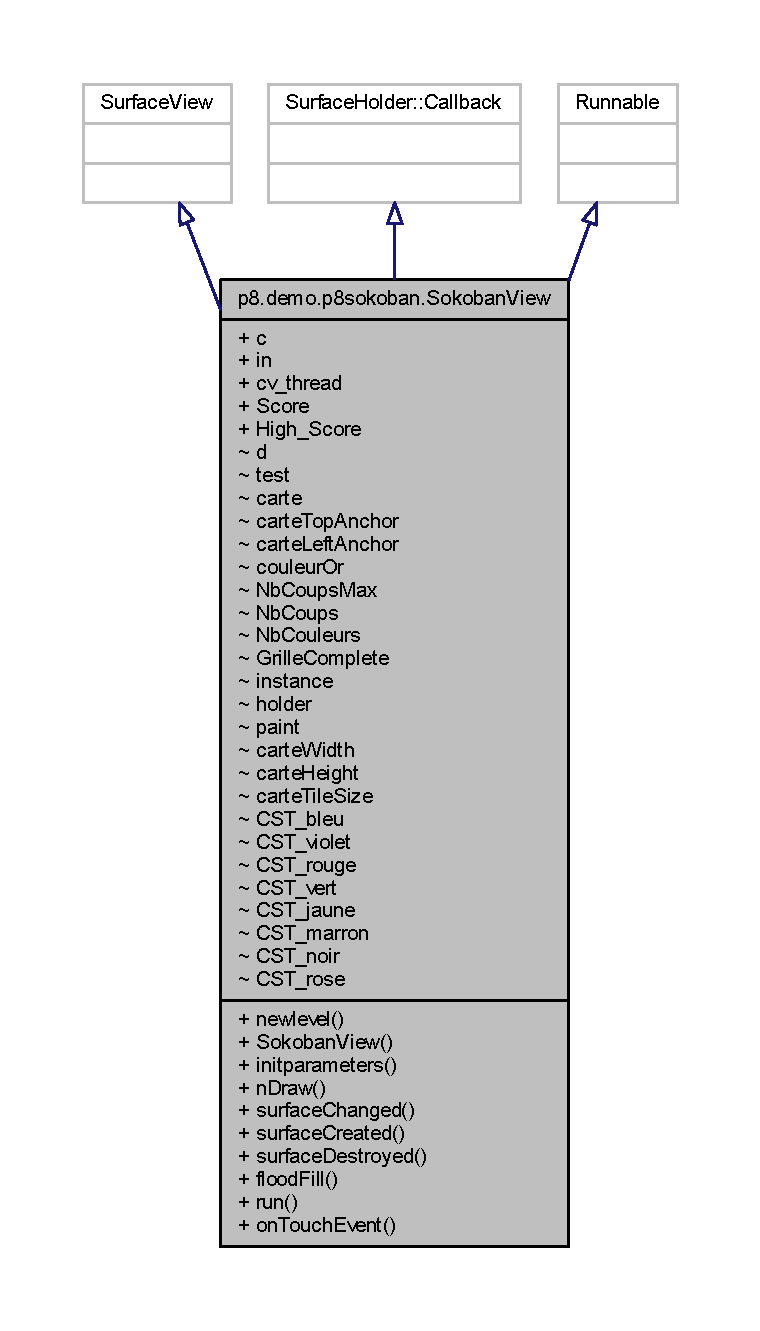
\includegraphics[height=550pt]{classp8_1_1demo_1_1p8sokoban_1_1_sokoban_view__inherit__graph}
\end{center}
\end{figure}


Graphe de collaboration de p8.\+demo.\+p8sokoban.\+Sokoban\+View\+:
\nopagebreak
\begin{figure}[H]
\begin{center}
\leavevmode
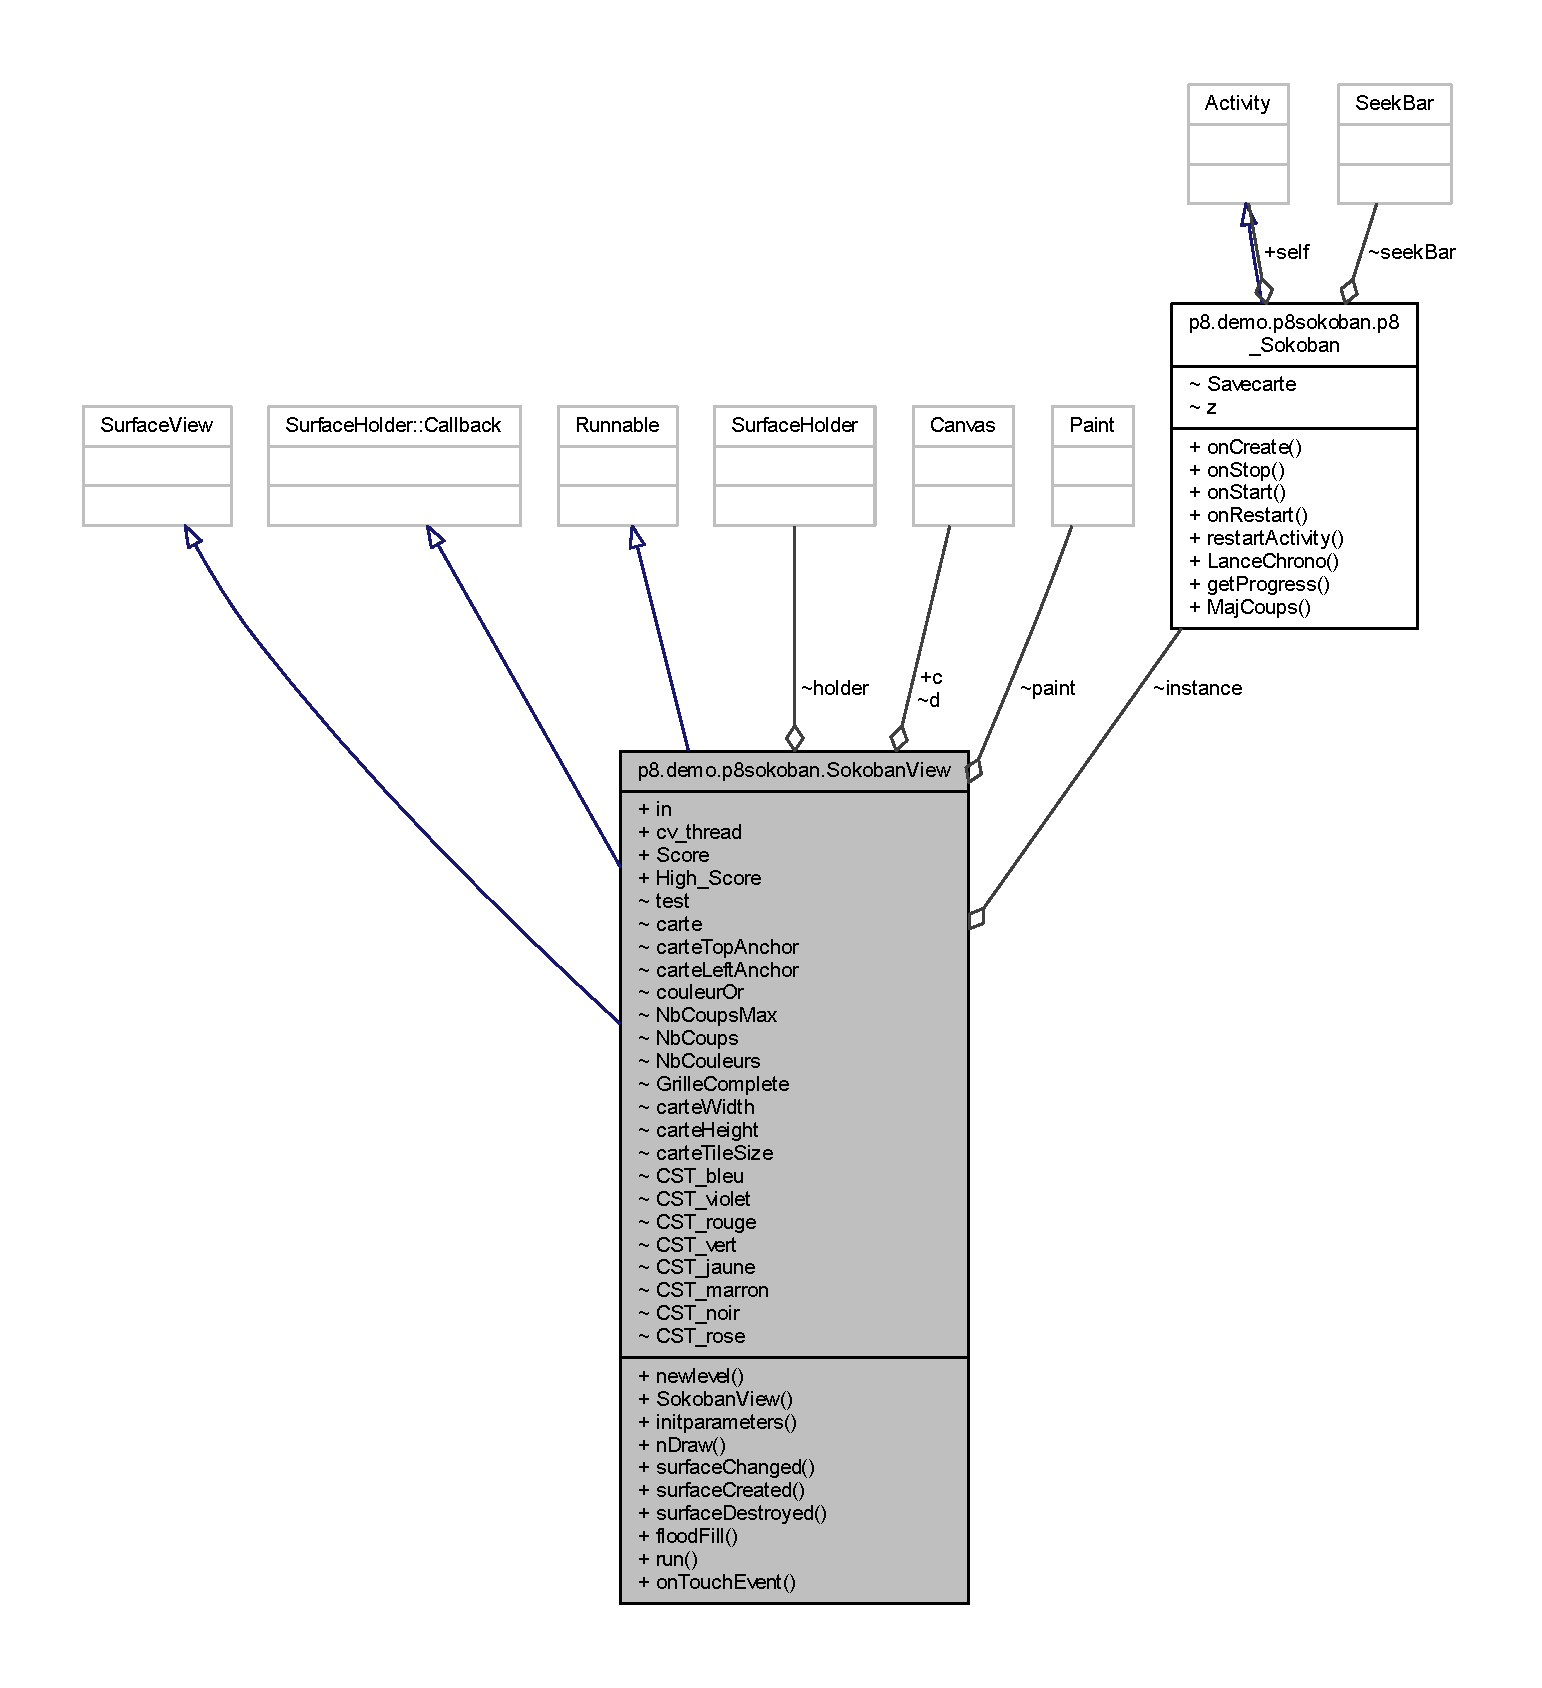
\includegraphics[width=350pt]{classp8_1_1demo_1_1p8sokoban_1_1_sokoban_view__coll__graph}
\end{center}
\end{figure}
\subsection*{Fonctions membres publiques}
\begin{DoxyCompactItemize}
\item 
void \hyperlink{classp8_1_1demo_1_1p8sokoban_1_1_sokoban_view_a589ccb831a549d7c328418e038c7bb4c}{newlevel} (int Nombre\+Couleurs)
\item 
\hyperlink{classp8_1_1demo_1_1p8sokoban_1_1_sokoban_view_a9b77c402af6779c46c11e0bd6572eeec}{Sokoban\+View} (Context context, Attribute\+Set attrs)
\item 
void \hyperlink{classp8_1_1demo_1_1p8sokoban_1_1_sokoban_view_aae2d77f292a6cc7b5e4b68f0c8df0243}{initparameters} ()
\item 
void \hyperlink{classp8_1_1demo_1_1p8sokoban_1_1_sokoban_view_a162eb9585b545f2c922d6d2aba411d68}{n\+Draw} (Canvas canvas)
\item 
void \hyperlink{classp8_1_1demo_1_1p8sokoban_1_1_sokoban_view_a6f555dde84f49e730114c5585e444e2b}{surface\+Changed} (Surface\+Holder holder, int format, int width, int height)
\item 
void \hyperlink{classp8_1_1demo_1_1p8sokoban_1_1_sokoban_view_a4b9325992cfbf98b878f11b75909edac}{surface\+Created} (Surface\+Holder arg0)
\item 
void \hyperlink{classp8_1_1demo_1_1p8sokoban_1_1_sokoban_view_a0b190fc3dd3e36091c512adb6d827172}{surface\+Destroyed} (Surface\+Holder arg0)
\item 
void \hyperlink{classp8_1_1demo_1_1p8sokoban_1_1_sokoban_view_a2978b3f19073d8b08ec5ad612dd1be23}{flood\+Fill} (int x, int y, int Ancienne\+Couleur, int Nouvelle\+Couleur)
\item 
void \hyperlink{classp8_1_1demo_1_1p8sokoban_1_1_sokoban_view_a6c6c4a3e01b49c9b46fbf698eda4ad5a}{run} ()
\item 
boolean \hyperlink{classp8_1_1demo_1_1p8sokoban_1_1_sokoban_view_a7447a5c085cc25b6be162b832a358700}{on\+Touch\+Event} (Motion\+Event event)
\end{DoxyCompactItemize}
\subsection*{Attributs publics}
\begin{DoxyCompactItemize}
\item 
\hypertarget{classp8_1_1demo_1_1p8sokoban_1_1_sokoban_view_adc4918b7a35d3b66e35634a91c3d177e}{}Canvas {\bfseries c}\label{classp8_1_1demo_1_1p8sokoban_1_1_sokoban_view_adc4918b7a35d3b66e35634a91c3d177e}

\item 
\hypertarget{classp8_1_1demo_1_1p8sokoban_1_1_sokoban_view_a8687c2a2d608dca85e54f1d961cce7f5}{}boolean {\bfseries in} = true\label{classp8_1_1demo_1_1p8sokoban_1_1_sokoban_view_a8687c2a2d608dca85e54f1d961cce7f5}

\item 
\hypertarget{classp8_1_1demo_1_1p8sokoban_1_1_sokoban_view_a50614f7a9544e6f522cb166bc7e81208}{}Thread {\bfseries cv\+\_\+thread}\label{classp8_1_1demo_1_1p8sokoban_1_1_sokoban_view_a50614f7a9544e6f522cb166bc7e81208}

\end{DoxyCompactItemize}
\subsection*{Attributs publics statiques}
\begin{DoxyCompactItemize}
\item 
\hypertarget{classp8_1_1demo_1_1p8sokoban_1_1_sokoban_view_aa04bdcb5159dd484c318536e75644661}{}static int {\bfseries Score} =0\label{classp8_1_1demo_1_1p8sokoban_1_1_sokoban_view_aa04bdcb5159dd484c318536e75644661}

\item 
\hypertarget{classp8_1_1demo_1_1p8sokoban_1_1_sokoban_view_a3c41b8c3e28c47feab2b45315493d729}{}static int {\bfseries High\+\_\+\+Score} =0\label{classp8_1_1demo_1_1p8sokoban_1_1_sokoban_view_a3c41b8c3e28c47feab2b45315493d729}

\end{DoxyCompactItemize}


\subsection{Documentation des constructeurs et destructeur}
\hypertarget{classp8_1_1demo_1_1p8sokoban_1_1_sokoban_view_a9b77c402af6779c46c11e0bd6572eeec}{}\index{p8\+::demo\+::p8sokoban\+::\+Sokoban\+View@{p8\+::demo\+::p8sokoban\+::\+Sokoban\+View}!Sokoban\+View@{Sokoban\+View}}
\index{Sokoban\+View@{Sokoban\+View}!p8\+::demo\+::p8sokoban\+::\+Sokoban\+View@{p8\+::demo\+::p8sokoban\+::\+Sokoban\+View}}
\subsubsection[{Sokoban\+View(\+Context context, Attribute\+Set attrs)}]{\setlength{\rightskip}{0pt plus 5cm}p8.\+demo.\+p8sokoban.\+Sokoban\+View.\+Sokoban\+View (
\begin{DoxyParamCaption}
\item[{Context}]{context, }
\item[{Attribute\+Set}]{attrs}
\end{DoxyParamCaption}
)}\label{classp8_1_1demo_1_1p8sokoban_1_1_sokoban_view_a9b77c402af6779c46c11e0bd6572eeec}
The constructor called from the main Jet\+Boy activity


\begin{DoxyParams}{Paramètres}
{\em context} & \\
\hline
{\em attrs} & \\
\hline
\end{DoxyParams}


\subsection{Documentation des fonctions membres}
\hypertarget{classp8_1_1demo_1_1p8sokoban_1_1_sokoban_view_a2978b3f19073d8b08ec5ad612dd1be23}{}\index{p8\+::demo\+::p8sokoban\+::\+Sokoban\+View@{p8\+::demo\+::p8sokoban\+::\+Sokoban\+View}!flood\+Fill@{flood\+Fill}}
\index{flood\+Fill@{flood\+Fill}!p8\+::demo\+::p8sokoban\+::\+Sokoban\+View@{p8\+::demo\+::p8sokoban\+::\+Sokoban\+View}}
\subsubsection[{flood\+Fill(int x, int y, int Ancienne\+Couleur, int Nouvelle\+Couleur)}]{\setlength{\rightskip}{0pt plus 5cm}void p8.\+demo.\+p8sokoban.\+Sokoban\+View.\+flood\+Fill (
\begin{DoxyParamCaption}
\item[{int}]{x, }
\item[{int}]{y, }
\item[{int}]{Ancienne\+Couleur, }
\item[{int}]{Nouvelle\+Couleur}
\end{DoxyParamCaption}
)}\label{classp8_1_1demo_1_1p8sokoban_1_1_sokoban_view_a2978b3f19073d8b08ec5ad612dd1be23}
Méthode principale qui contient le coeur du jeu C\textquotesingle{}est une méthode récursive qui permet de rechercher les cases de la même couleur que la première case et de les changer avec la nouvelle couleur qu\textquotesingle{}on a sélectionnée La recherche se fait récursivement en vérifiant les quatre cases qui se trouvent autour de la case courante 
\begin{DoxyParams}{Paramètres}
{\em x} & \\
\hline
{\em y} & \\
\hline
{\em Ancienne\+Couleur} & \\
\hline
{\em Nouvelle\+Couleur} & \\
\hline
\end{DoxyParams}
\hypertarget{classp8_1_1demo_1_1p8sokoban_1_1_sokoban_view_aae2d77f292a6cc7b5e4b68f0c8df0243}{}\index{p8\+::demo\+::p8sokoban\+::\+Sokoban\+View@{p8\+::demo\+::p8sokoban\+::\+Sokoban\+View}!initparameters@{initparameters}}
\index{initparameters@{initparameters}!p8\+::demo\+::p8sokoban\+::\+Sokoban\+View@{p8\+::demo\+::p8sokoban\+::\+Sokoban\+View}}
\subsubsection[{initparameters()}]{\setlength{\rightskip}{0pt plus 5cm}void p8.\+demo.\+p8sokoban.\+Sokoban\+View.\+initparameters (
\begin{DoxyParamCaption}
{}
\end{DoxyParamCaption}
)}\label{classp8_1_1demo_1_1p8sokoban_1_1_sokoban_view_aae2d77f292a6cc7b5e4b68f0c8df0243}
Initialisation du jeu \hypertarget{classp8_1_1demo_1_1p8sokoban_1_1_sokoban_view_a162eb9585b545f2c922d6d2aba411d68}{}\index{p8\+::demo\+::p8sokoban\+::\+Sokoban\+View@{p8\+::demo\+::p8sokoban\+::\+Sokoban\+View}!n\+Draw@{n\+Draw}}
\index{n\+Draw@{n\+Draw}!p8\+::demo\+::p8sokoban\+::\+Sokoban\+View@{p8\+::demo\+::p8sokoban\+::\+Sokoban\+View}}
\subsubsection[{n\+Draw(\+Canvas canvas)}]{\setlength{\rightskip}{0pt plus 5cm}void p8.\+demo.\+p8sokoban.\+Sokoban\+View.\+n\+Draw (
\begin{DoxyParamCaption}
\item[{Canvas}]{canvas}
\end{DoxyParamCaption}
)}\label{classp8_1_1demo_1_1p8sokoban_1_1_sokoban_view_a162eb9585b545f2c922d6d2aba411d68}
Méthode qui permet de dessiner toute la surface du jeu en appelant les méthodes paint... vues précédemment 
\begin{DoxyParams}{Paramètres}
{\em canvas} & \\
\hline
\end{DoxyParams}
\hypertarget{classp8_1_1demo_1_1p8sokoban_1_1_sokoban_view_a589ccb831a549d7c328418e038c7bb4c}{}\index{p8\+::demo\+::p8sokoban\+::\+Sokoban\+View@{p8\+::demo\+::p8sokoban\+::\+Sokoban\+View}!newlevel@{newlevel}}
\index{newlevel@{newlevel}!p8\+::demo\+::p8sokoban\+::\+Sokoban\+View@{p8\+::demo\+::p8sokoban\+::\+Sokoban\+View}}
\subsubsection[{newlevel(int Nombre\+Couleurs)}]{\setlength{\rightskip}{0pt plus 5cm}void p8.\+demo.\+p8sokoban.\+Sokoban\+View.\+newlevel (
\begin{DoxyParamCaption}
\item[{int}]{Nombre\+Couleurs}
\end{DoxyParamCaption}
)}\label{classp8_1_1demo_1_1p8sokoban_1_1_sokoban_view_a589ccb831a549d7c328418e038c7bb4c}
Génère la grille de jeu aléatoirement en generant deux nombres entre 0 et 12 pour remplir le tableau (grille) en generant un autre nombre aleatoire entre 0 et 7 ensuite on place les couleurs sur la grille selon la valeur de nb\+Aleat tant que la grille n\textquotesingle{}est pas remplie 
\begin{DoxyParams}{Paramètres}
{\em Nombre\+Couleurs} & \\
\hline
\end{DoxyParams}
\hypertarget{classp8_1_1demo_1_1p8sokoban_1_1_sokoban_view_a7447a5c085cc25b6be162b832a358700}{}\index{p8\+::demo\+::p8sokoban\+::\+Sokoban\+View@{p8\+::demo\+::p8sokoban\+::\+Sokoban\+View}!on\+Touch\+Event@{on\+Touch\+Event}}
\index{on\+Touch\+Event@{on\+Touch\+Event}!p8\+::demo\+::p8sokoban\+::\+Sokoban\+View@{p8\+::demo\+::p8sokoban\+::\+Sokoban\+View}}
\subsubsection[{on\+Touch\+Event(\+Motion\+Event event)}]{\setlength{\rightskip}{0pt plus 5cm}boolean p8.\+demo.\+p8sokoban.\+Sokoban\+View.\+on\+Touch\+Event (
\begin{DoxyParamCaption}
\item[{Motion\+Event}]{event}
\end{DoxyParamCaption}
)}\label{classp8_1_1demo_1_1p8sokoban_1_1_sokoban_view_a7447a5c085cc25b6be162b832a358700}
Méthode permettant de récuperer les évenements tactiles Appui sur le bouton \char`\"{}\+Commencer la partie\char`\"{}, lancement du jeu et du chrono Appui sur les boutons de couleurs, la gestion de la couleur des cases, l\textquotesingle{}affichage du score, du nombre de coups Tant que la grille n\textquotesingle{}est pas completée avec la meme couleur, on continue 
\begin{DoxyParams}{Paramètres}
{\em event} & \\
\hline
\end{DoxyParams}
\begin{DoxyReturn}{Renvoie}

\end{DoxyReturn}
\hypertarget{classp8_1_1demo_1_1p8sokoban_1_1_sokoban_view_a6c6c4a3e01b49c9b46fbf698eda4ad5a}{}\index{p8\+::demo\+::p8sokoban\+::\+Sokoban\+View@{p8\+::demo\+::p8sokoban\+::\+Sokoban\+View}!run@{run}}
\index{run@{run}!p8\+::demo\+::p8sokoban\+::\+Sokoban\+View@{p8\+::demo\+::p8sokoban\+::\+Sokoban\+View}}
\subsubsection[{run()}]{\setlength{\rightskip}{0pt plus 5cm}void p8.\+demo.\+p8sokoban.\+Sokoban\+View.\+run (
\begin{DoxyParamCaption}
{}
\end{DoxyParamCaption}
)}\label{classp8_1_1demo_1_1p8sokoban_1_1_sokoban_view_a6c6c4a3e01b49c9b46fbf698eda4ad5a}
run (run du thread cree) on endort le thread, on modifie le compteur d\textquotesingle{}animation, on prend la main pour dessiner et on dessine puis on libere le canvas \hypertarget{classp8_1_1demo_1_1p8sokoban_1_1_sokoban_view_a6f555dde84f49e730114c5585e444e2b}{}\index{p8\+::demo\+::p8sokoban\+::\+Sokoban\+View@{p8\+::demo\+::p8sokoban\+::\+Sokoban\+View}!surface\+Changed@{surface\+Changed}}
\index{surface\+Changed@{surface\+Changed}!p8\+::demo\+::p8sokoban\+::\+Sokoban\+View@{p8\+::demo\+::p8sokoban\+::\+Sokoban\+View}}
\subsubsection[{surface\+Changed(\+Surface\+Holder holder, int format, int width, int height)}]{\setlength{\rightskip}{0pt plus 5cm}void p8.\+demo.\+p8sokoban.\+Sokoban\+View.\+surface\+Changed (
\begin{DoxyParamCaption}
\item[{Surface\+Holder}]{holder, }
\item[{int}]{format, }
\item[{int}]{width, }
\item[{int}]{height}
\end{DoxyParamCaption}
)}\label{classp8_1_1demo_1_1p8sokoban_1_1_sokoban_view_a6f555dde84f49e730114c5585e444e2b}
Callback sur le cycle de vie de la surfaceview \hypertarget{classp8_1_1demo_1_1p8sokoban_1_1_sokoban_view_a4b9325992cfbf98b878f11b75909edac}{}\index{p8\+::demo\+::p8sokoban\+::\+Sokoban\+View@{p8\+::demo\+::p8sokoban\+::\+Sokoban\+View}!surface\+Created@{surface\+Created}}
\index{surface\+Created@{surface\+Created}!p8\+::demo\+::p8sokoban\+::\+Sokoban\+View@{p8\+::demo\+::p8sokoban\+::\+Sokoban\+View}}
\subsubsection[{surface\+Created(\+Surface\+Holder arg0)}]{\setlength{\rightskip}{0pt plus 5cm}void p8.\+demo.\+p8sokoban.\+Sokoban\+View.\+surface\+Created (
\begin{DoxyParamCaption}
\item[{Surface\+Holder}]{arg0}
\end{DoxyParamCaption}
)}\label{classp8_1_1demo_1_1p8sokoban_1_1_sokoban_view_a4b9325992cfbf98b878f11b75909edac}
Callback sur le score a afficher \hypertarget{classp8_1_1demo_1_1p8sokoban_1_1_sokoban_view_a0b190fc3dd3e36091c512adb6d827172}{}\index{p8\+::demo\+::p8sokoban\+::\+Sokoban\+View@{p8\+::demo\+::p8sokoban\+::\+Sokoban\+View}!surface\+Destroyed@{surface\+Destroyed}}
\index{surface\+Destroyed@{surface\+Destroyed}!p8\+::demo\+::p8sokoban\+::\+Sokoban\+View@{p8\+::demo\+::p8sokoban\+::\+Sokoban\+View}}
\subsubsection[{surface\+Destroyed(\+Surface\+Holder arg0)}]{\setlength{\rightskip}{0pt plus 5cm}void p8.\+demo.\+p8sokoban.\+Sokoban\+View.\+surface\+Destroyed (
\begin{DoxyParamCaption}
\item[{Surface\+Holder}]{arg0}
\end{DoxyParamCaption}
)}\label{classp8_1_1demo_1_1p8sokoban_1_1_sokoban_view_a0b190fc3dd3e36091c512adb6d827172}
Callback sur le highscore et sa sauvegarde 

La documentation de cette classe a été générée à partir du fichier suivant \+:\begin{DoxyCompactItemize}
\item 
app/src/main/java/p8/demo/p8sokoban/Sokoban\+View.\+java\end{DoxyCompactItemize}

%--- End generated contents ---

% Index
\backmatter
\newpage
\phantomsection
\clearemptydoublepage
\addcontentsline{toc}{chapter}{Index}
\printindex

\end{document}
